%% Sets aspect ratio to 16:10, and frame size to 160mm by 100mm
% Please, do not use old-school 4:3 ratio anymore:)
\documentclass[aspectratio=1610]{beamer}
% všechny soubory jsou v utf-8
\usepackage{ucs}% pro kódování UTF-8
\PrerenderUnicode{ěščřžýáíéĚŠČŘŽÝÁÍÉďťňĎŤŇůúÚóÓ} % předkreslení diakritiky, možno přidat/ubrat znaky podle potřeby	

%% Select your favorite language
%\usepackage[english]{babel} % Multilingual support for LaTeX
\usepackage[czech]{babel}
\usepackage[IL2]{fontenc}% csr fonty (pokud jsou nainstalovány česká postscriptová mísma)

\usepackage[utf8]{inputenc} % Accept different input encodings
\usepackage{graphicx} % Enhanced support for graphics
\usepackage{listings} % Typeset source code listings using LaTeX
\usepackage{color} % Colour control for LaTeX documents
\usepackage{bm} % Colour control for LaTeX documents

%% Copy your favorite logo from "vut_logo_archive/" to root folder 
% and rename file to "logo.png"

%% Select color theme
\usepackage[FSI]{themevut}

\usepackage{parskip}
\usepackage{media9}	
% ----------------------------------------------------------------------
% TITLE PAGE
% ----------------------------------------------------------------------

% The short title appears at the bottom of every slide, the full title
% is only on the title page.
\title[Sémantická segmentace obrazu pomocí CNN]
{Sémantická segmentace obrazu pomocí konvolučních neuronových sítí}

% Type of project, i.e. Bachelor, Master, PhD, etc.
\subtitle
{Diplomová práce}

% Your name
\author[Bc. Filip Špila]
{Bc. Filip Špila \\
	\texttt{filipspila@gmail.com}}

% Your institution
\institute
{Ústav mechaniky těles, mechatroniky a biomechaniky \\
	Vysoké učení technické v Brně
}

% Date, can be changed to a custom date
\date{\today}

% Logo on title page
\titlegraphic{
\includegraphics[height=.1\textheight]{logo4.png}}

\begin{document}
	
	% ----------------------------------------------------------------------
	% PRESENTATION SLIDES
	% ----------------------------------------------------------------------
	
	\begin{frame}
	% Print the title page as the first slide
	\titlepage
\end{frame}

% ----------------------------------------------------------------------
% https://cs.overleaf.com/learn/latex/Lists

\begin{frame}{Cíle práce}
	\begin{enumerate}
		\item Nastudování problematiky segmentace obrazu pomocí konvolučních neuronových sítí
		\item Výběr perspektivní architektury sítě spolu s její implementací
		\item Vytvoření vlastní trénovací množiny obrázků
		\item Vytvoření segmentovaného obrazu
		\item Vyhodnocení úspěšnosti segmentace
	\end{enumerate}	
\end{frame}

% ----------------------------------------------------------------------

\begin{frame}{Sémantická segmentace}
	\textbf{Cíle sémantické segmentace}
	\begin{itemize}
	\item Přiřadit každému pixelu v obrázku právě jednu třídu objektu (auto, člověk, zvíře, ...)
	% Narozdil od klasifikace obrazu jako celku
	\item Provádět segmentaci co nejpřesněji
	% Tedy s presnym vykreslenim hranice kazdeho objektu
	\item Zajistit, aby algoritmus uměl generalizovat
	% Tedy aby spravne klasifikoval objekty bez ohledu na svetelne podminky, ruzne nedokonalosti atp.	
	\end{itemize}
	\vspace{5mm}		
	\begin{center}
		\begin{figure}
			\includemedia[
			width=0.4\linewidth,
			height=0.2\linewidth,
			addresource=cut.mp4,
			activate=pagevisible,
			passcontext, 
			playbutton=none,
			flashvars={				
				source=cut.mp4
				&autoPlay=true
				&loop=false
			}
			]{}{VPlayer.swf}
		\caption{Sémantická segmentace}
		\end{figure}	
	\end{center}
\end{frame}
% ----------------------------------------------------------------------
% https://en.wikibooks.org/wiki/LaTeX/Floats,_Figures_and_Captions
\begin{frame}{Neuronové sítě a učení s učitelem}
	\textbf{Úloha neuronové sítě}
	\begin{itemize}
		\item Aproximace obecné funkce $y=f(x;\phi)$ funkcí $ y^* = f^*(x;\phi)	$ řešením:					
		\begin{gather}
		\phi \leftarrow \, \text{arg min} \, L(y, f^*(x;\phi))	
		\end{gather} 
		 		
		\noindent kde $ \phi $ jsou trénovatelné parametry. \\~\\
		Funkce $ L $ se nazývá \textbf{hodnotící funkce}. Parametry $ \phi $ jsou nalezeny učením sítě \\ tzv. \textbf{učením s učitelem}.
		
	\end{itemize}
\end{frame}
% ----------------------------------------------------------------------
% https://en.wikibooks.org/wiki/LaTeX/Floats,_Figures_and_Captions
\begin{frame}{Neuronové sítě a učení s učitelem}
\textbf{Proč pro segmentaci místo klasických metod použít neuronovou síť?}
\begin{itemize}
	\item Dovede velmi dobře aproximovat silně nelineární funkce
	\item Potřebuje jen mírně předzpracovaná data
	\item Detekuje obecné vzory v datech = dovede lépe generalizovat
	\item Algoritmus je robustnější
	
\end{itemize}
\end{frame}
% ----------------------------------------------------------------------
\begin{frame}{Úloha klasifikace}
\begin{columns}
	\column{0.45\textwidth}
	\textbf{Definice klasifikační úlohy}
	\vspace{3mm}
	\begin{itemize}
		\item Aproximovaná funkce nabývá pouze určitých diskrétních hodnot
	\end{itemize}
	\begin{gather}
	f(x_1,x_2;\phi) = 
	\begin{cases}	
	1\\
	-1  
	\end{cases} 
	\end{gather}	
	\column{0.45\textwidth}
	\begin{figure}[h]
		\begin{center}
			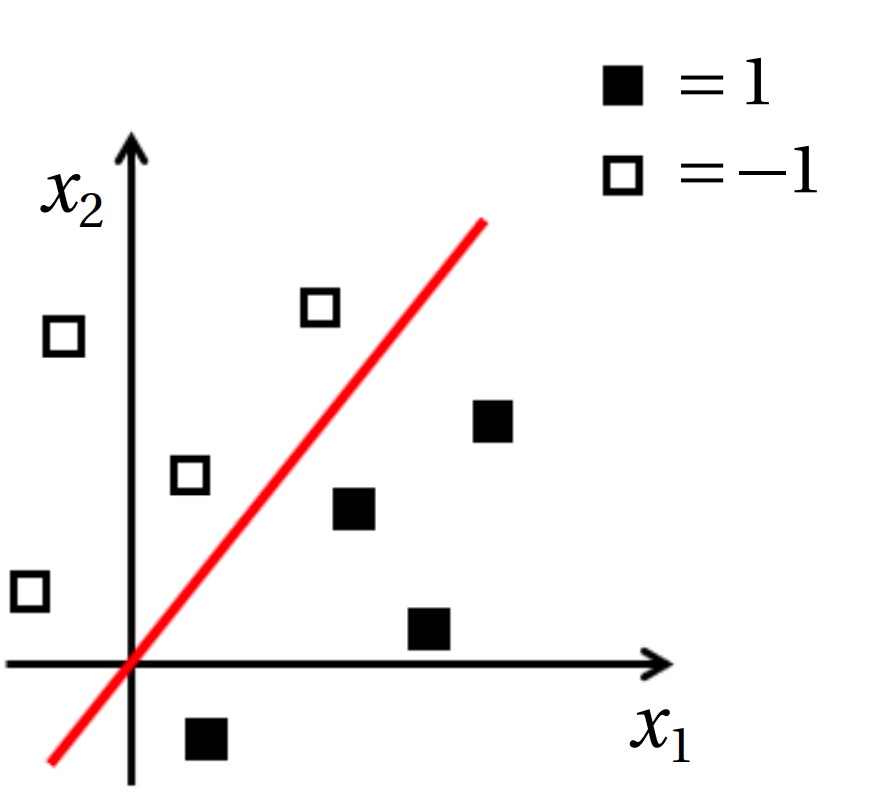
\includegraphics[width=5cm, keepaspectratio]{linsep.png}
		\end{center}
		\caption{Úloha klasifikace} 	
	\end{figure}
\end{columns}	

\end{frame}
% ----------------------------------------------------------------------
\begin{frame}{CNN - konvoluční neuronové sítě}
	\begin{figure}[h]
	\begin{center}
		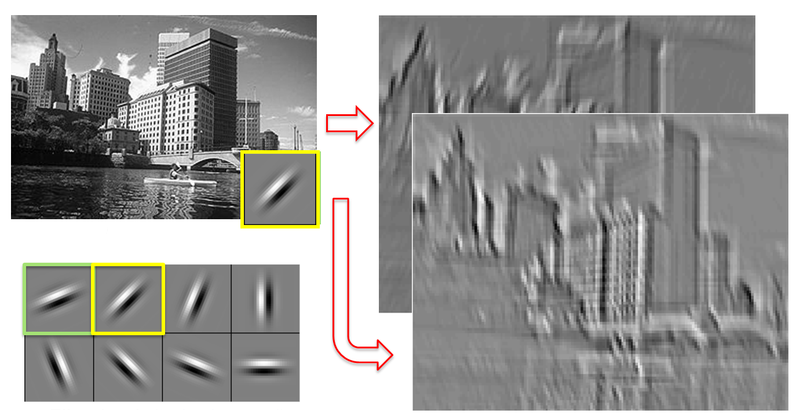
\includegraphics[width=12cm, keepaspectratio]{maps2.png}
	\end{center}
	\caption{Mapy prvků v obraze} 	
\end{figure}
\end{frame}
% ----------------------------------------------------------------------
\begin{frame}{CNN - konvoluční neuronové sítě}
\begin{figure}[h]
	\begin{center}
		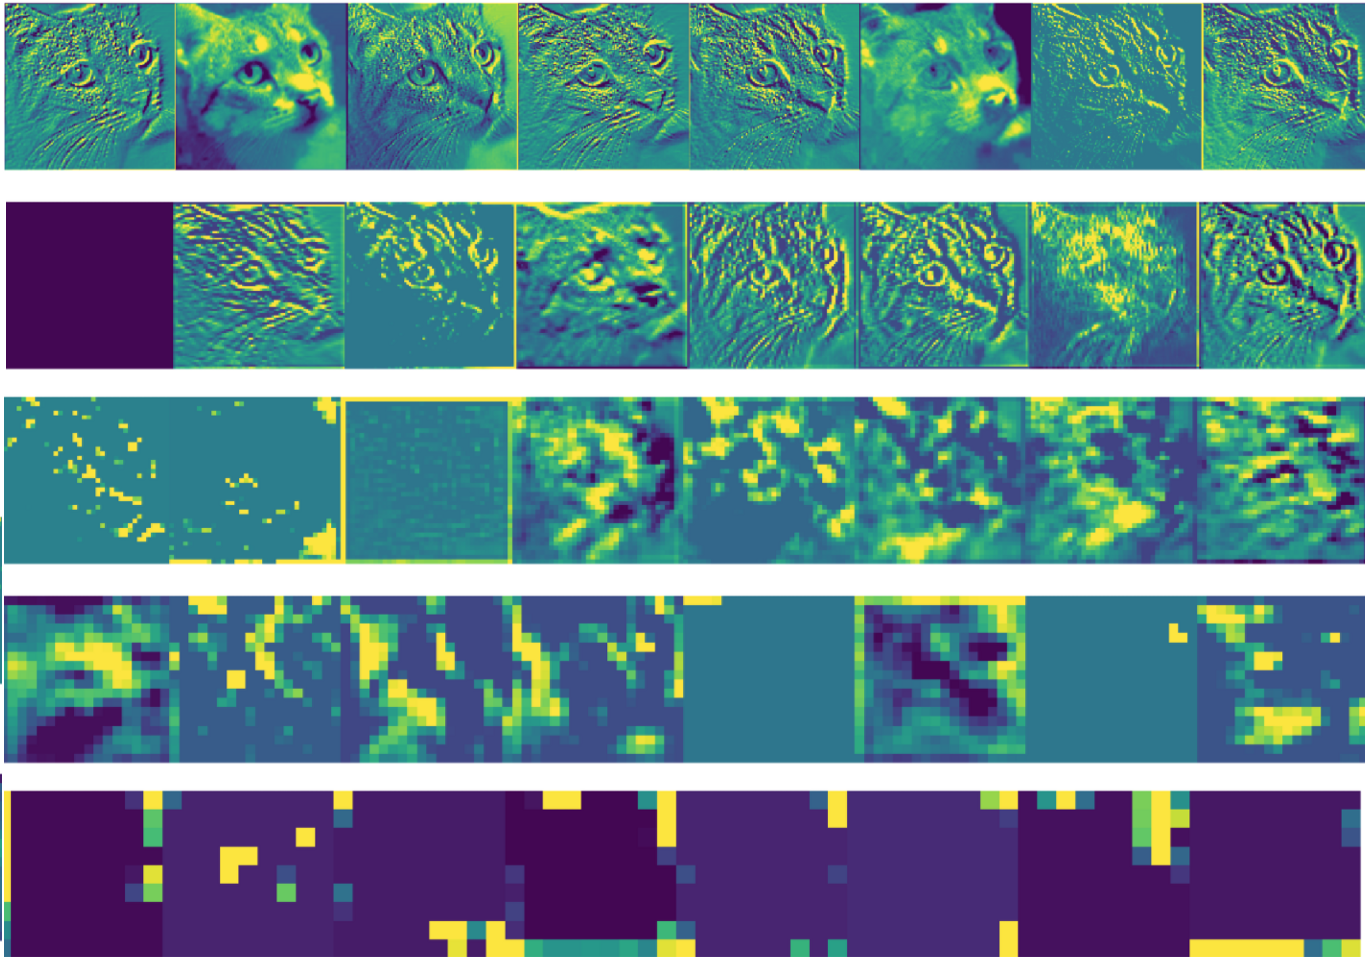
\includegraphics[width=10cm, keepaspectratio]{maps.png}
	\end{center}
	\caption{Mapy prvků v obraze} 	
\end{figure}
\end{frame}
% ----------------------------------------------------------------------
\begin{frame}{CNN - konvoluční neuronové sítě}
\begin{figure}[h]
	\begin{center}
		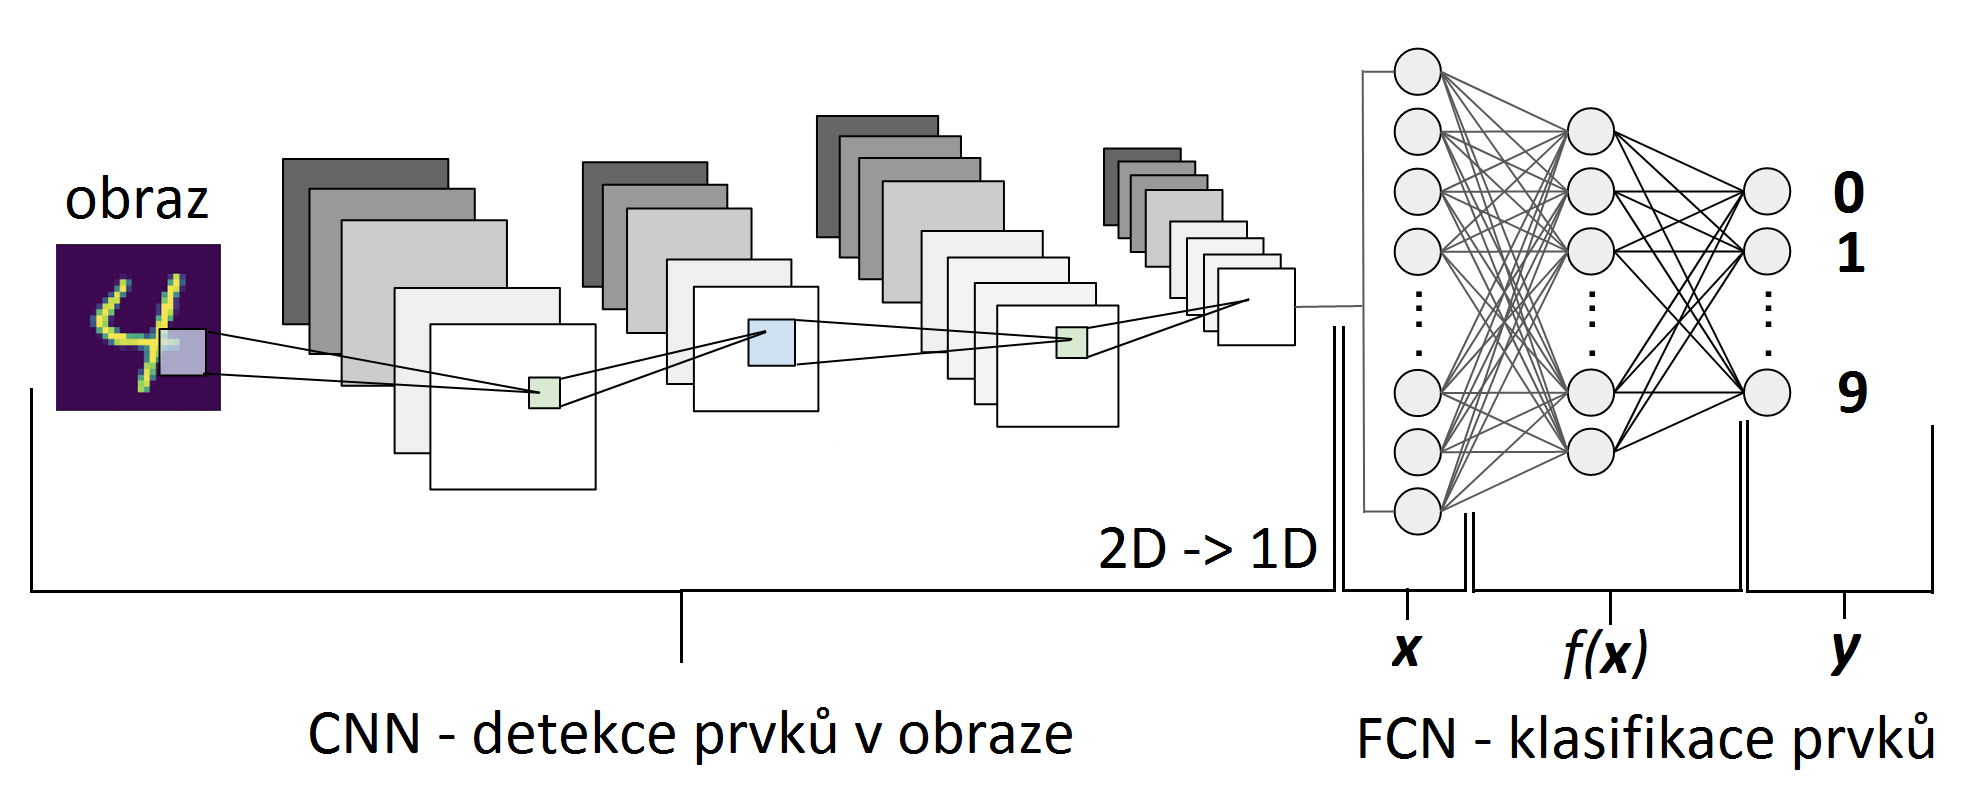
\includegraphics[width=15cm, keepaspectratio]{cnn.png}
	\end{center}
	\caption{Úloha klasifikace} 	
\end{figure}
\end{frame}
% ----------------------------------------------------------------------
\begin{frame}{Segmentace - architektura enkodér-dekodér}
\begin{figure}[h]
	\begin{center}
		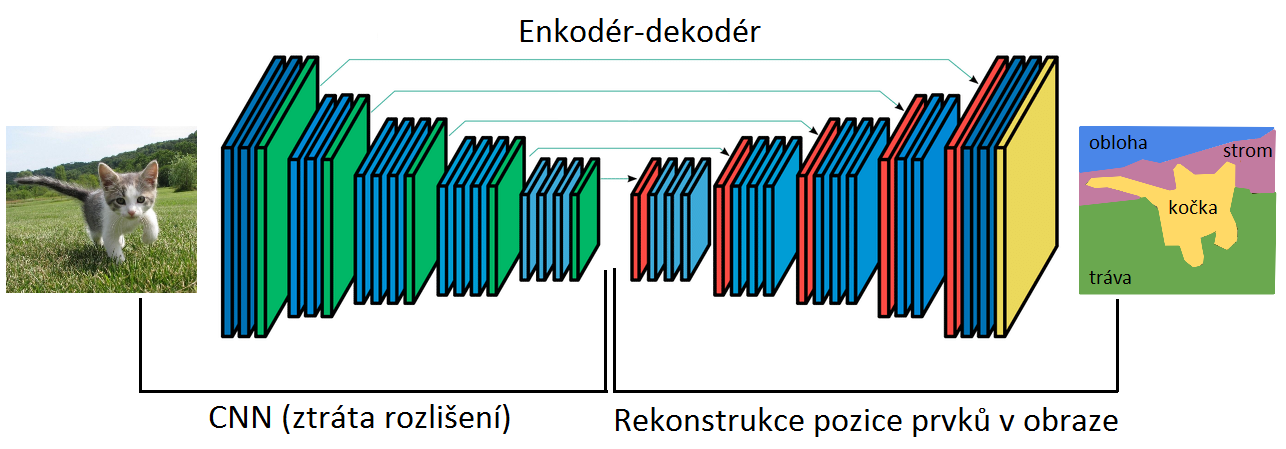
\includegraphics[width=15cm, keepaspectratio]{segnet.png}
	\end{center}
	\caption{Architektura enkodér-dekodér} 	
\end{figure}
\end{frame}
% ----------------------------------------------------------------------
% https://en.wikibooks.org/wiki/LaTeX/Tables
\begin{frame}{Table}
\begin{center}
\begin{table}
\caption{Your caption}
\begin{tabular}{l | c | c | c | r}
\textbf{Function name} & \textbf{Duration} & \textbf{Complexity} & \textbf{Length} & \textbf{Score}\\
\hline \hline
Algo 1 & 0.0159 & 0.50 & 125 & 78 \\
Algo 2 & 0.0453 & 0.65 & 854 & 88 \\
Algo 3 & 0.8642 & 0.77 &  84 & 95 \\
Algo 4 & 0.0020 & 0.24 & 638 & 76 \\
\end{tabular}
\end{table}
\end{center}
\end{frame}
% ----------------------------------------------------------------------
% It is a common practice you already have reviewer(s) comments/questions before your presentation. Sometimes, it is useful to prepare extra slides to answer those questions.
\begin{frame}{Reviewer's questions}
\begin{columns}
\column{0.45\textwidth}
\begin{exampleblock}{Question 1}
Lorem ipsum dolor sit amet, consectetur adipiscing elit. Integer lectus nisl, ultricies in feugiat rutrum, porttitor sit amet augue. Aliquam ut tortor mauris. Sed volutpat ante purus, quis accumsan dolor.
\end{exampleblock}

\column{0.45\textwidth}
\begin{block}{Answer 1}
Lorem ipsum dolor sit amet, consectetur adipiscing elit. Integer lectus nisl, ultricies in feugiat rutrum, porttitor sit amet augue. Aliquam ut tortor mauris. Sed volutpat ante purus, quis accumsan dolor.
\end{block}
\end{columns}
\end{frame}

% ----------------------------------------------------------------------

\end{document}
